One of the most crucial steps to be taken before the design of the reference architecture was the analysis of the source code of the DBT project. Thus, this section describes in detail all the software modules identified as well as their role in the final model. 

In a prime instance, it was used a static code analysis tool called \textit{Understand\textsuperscript{TM}} to help to fully comprehend the DBT source code. Among several features, \textit{Understand} provides pertinent information regarding the code and it can be used to easily check the contents and interactions between functions, classes, variables and others. After organizing all the source files in folders and creating a project in \textit{Understand}, the result was as follows:        
 
\begin{figure}[!hb]
\centerline{
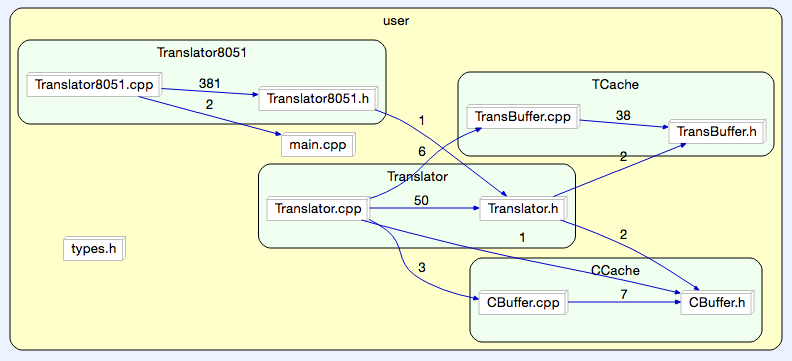
\includegraphics[scale=0.55]{images/understand}}
\caption{DBT Dependency Graph.}
\label{fig:understand} 
\end{figure}

Figure \ref{fig:understand} shows a dependency analysis of the DBT project. Each block highlighted in green contains source and header files, which enclosure a C++ class: \textbf{CBuffer}, \textbf{CTransBuffer}, \textbf{CTranslator} and \textbf{CTranslator8051}. Based on the dependencies observed, it was possible to follow a flow of the code analysis. The major goal at this point was to enhance all the \textbf{components} and find the possible \textbf{interfaces} between them.

\newpage
\subsubsection*{CBuffer}

The \texttt{CBuffer} class (figure \ref{fig:cbufferclass}) is defined and implemented in \texttt{CBuffer.h} and \texttt{CBuffer.cpp}. It is mainly composed by pointers to source code (\texttt{baseBufferAddr} and \texttt{lastBufferAddr}) stored in memory and a method called \texttt{load()} that initializes these pointers with the respective addresses. It also stores the size of the buffer in a variable called \texttt{c\_size}. That being said, this software block can be considered as an \textbf{atomic component}, and the referred method together with the accessors for the memory can be identified has \textbf{services} provided from it.

\begin{figure}[!htb]
\centerline{
\includegraphics[scale=0.53]{images/Cbufferclass}}
\caption{CBuffer Class.}
\label{fig:cbufferclass} 
\end{figure}

\subsubsection*{CTransBuffer}

\texttt{CTransBuffer} class (figure \ref{fig:tbufferclass}) is defined and implemented in \texttt{TransBuffer.h} and \texttt{TransBuffer.cpp}. This class implements an hash table that maps the source code memory address of a Basic Block (key) to translated code memory addresses (value). 

\begin{figure}[!htb]
\centerline{
\includegraphics[scale=0.53]{images/CTransBufferclass}}
\caption{CTransBuffer Class.}
\label{fig:tbufferclass} 
\end{figure}

Like \texttt{CBuffer}, it contains as member variables pointers to the beginning and ending of target code (\texttt{pTargetMem\_begin} and \texttt{pTargetMem\_end}). It also has the address of the source code (\texttt{transSourAddr}) and tree relevant variables: one to store the size of the table (\texttt{t\_size}), another to update the size still available, and at last, the size of the basic block (\texttt{bb\_size}). As member methods, \texttt{TransCache} is composed by several functions used in accessing and managing the hash table (read and write operations) such as \texttt{getCacheAddr(), getCurrInsAddr(), getCodeSize(), addTag(), getTag(), getLastTransAddr(), getTransAddr(), checkForRoom()} and \texttt{cacheCode()}. All of these functions can be seen as services provided by this class to other modules of the code, therefore, \texttt{TrasnCache} is considered also an \textbf{atomic component} and the referred API a \textbf{service}.




\subsubsection*{Translator and Translator8051}

The following figure contains the definition of \texttt{CTranslator} and \texttt{CTranslator8051} classes, two classes that define and implements the engine of the translator together with the specific behavior for the source and target architectures. 

\begin{figure}[!htb]
\centerline{
\includegraphics[scale=0.53]{images/CTranslatorclass}}
\caption{CTranslator, CTranslator8051 and SourceEnvironment classes.}
\label{fig:translatorclass} 
\end{figure}


A new class identified in figure \ref{fig:translatorclass} is \texttt{SourceEnvironment}. This structure contains information about the execution environment of the source architecture, namely, the value of current \textbf{\textit{PC}} (that points to the source code) and another memory structure called \textbf{dataMem}, which represents the data memory of the 8051. Following the same ideas already presented for \texttt{CBuffer} and \texttt{CTransBuffer}, another possible \textbf{component} might be the \texttt{SourceEnvironment}, which provides access to the referred variables by other modules. 

The engine of the translator (translation and execution) is implemented in \texttt{CTranslator}. This class contains an instance of \texttt{CBuffer}, used to access the source code, an instance of \texttt{CTransBuffer}, used to store and read target code, and an instance of a class called \texttt{SourceEnvironment}, that contains information about the execution environment of the source architecture. Also, \texttt{CTranslator} contains another variables used in the engine and defined also for the derived class: \texttt{currBBExecPtr} (pointer to current translated BB), \texttt{eoExec} (flag that signalizes the end of execution) and \texttt{eoBB} (flag that signalizes the end of translation). As member methods the class contains several functions, all with specific functionalities: functions to start and run the DBT (\texttt{initTranslator()}, \texttt{sourceCodeLoader()} and \texttt{runDBT()}), a method responsible for translate BB (\texttt{translate()}), and pure virtual functions that must be overloaded accordingly with the source and target architecture: \texttt{decode()} and \texttt{gen\_prolog()} and \texttt{gen\_epilog()}. Since \texttt{CTranslator} is independent of the architectures and given its behavior as the engine of translation, another \textbf{component} identified is \texttt{DBTEngine}, composed by a \texttt{Translator} and \texttt{Executor}. 

Continuing with the analysis, the last class referred is \texttt{CTranslator8051}, a concrete class derived from \texttt{CTranslator} that implements specific behavior for both architecture. By so, the virtual functions defined in the base class are implemented. The \texttt{decode()} method is responsible for identifying and decoding the operands of the source instruction (specific for source architecture). For that, a set of callback functions were created (\texttt{fineDecode\_0x0(), fineDecode\_0x1()}, etc) each one specific for a type of instruction. At the end, these callbacks are responsible for calling functions used to generate the target code (target behavior), such us, \texttt{gen\_ld8(), gen\_st8()}, among others. All of these functions are used to generate intermediate representation (\textit{IR}) and target code, that is stored in \texttt{CTransBuffer}. Some auxiliary functions are used (helper function - \texttt{gen\_helper()}, etc) to those situations were the behavior is not easy to reproduce with straight assembly code.
Finally, the virtual functions \texttt{gen\_epilog()} \texttt{gen\_prolog()} must also be implemented in \texttt{CTranslator8051}. These function are specific for the target architecture since both insert \textit{ISA} specific code in \texttt{CTransCache} (code that ensures the saving of registers and return address - prologue - and code to restore the program state and flow).

That being said, it becomes easy to identified possible \textbf{components}. Since there are separated code associated with each architecture, two clusters (source and target) can be identified: the \texttt{Source Cluster} is mainly composed by a representation of the \texttt{Source Architecture}, a \texttt{Decoder} and a block representing the \texttt{Source Environments}, and the \texttt{Target Cluster} is composed also by a representation of the  \texttt{Target Architecture} and a  \texttt{Generator}.  

The next section presents a model for the top level component DBT and its subcomponents as well as the bindings between them. 
